\documentclass[Main.tex]{subfiles} 
\begin{document}

\subsubsection{Use Case 5: Test program realisering}
Test program Use Casen, er blevet udf�rdiget s�ledes at den fungerer som en simulator. N�r en bruger vil starte programmet, skal han f�rst v�lge om han vil bruge den rigtige robot, eller en simulering af robotten. Hvis simuleringen v�lges, bliver den klasse der har robotkaldene initialiseret med en simuleringsklasse af robotkaldene. P� den m�de bliver alle kald til robotfunktionerne simuleret, lige gyldigt om det er et brugerdefineret program eller standardprogrammet.\\
Kaldene til de robotfunktionerne, bliver simuleret s�ledes, at der bliver taget stilling til hvilke parametre der medsendes, og ud fra disse kan man se hvad mode robotten s�ttes til, om den rykker sig osv. Disse informationer logges s� til vinduet, samt til en logfil der ligger lokalt.\\
N�r brugeren logger ind med en simuleringsrobot, indl�ser systemet alle de programmer der er tilg�ngelige. Han har da mulighed for at k�re dem, og se n�jagtigt hvad der sker. Han kan ogs� pause, genstarte og stoppe en simulering. Derudover loader programmet ogs� alle simuleringslogs ind i en boks, der opdateres hver gang en simulering er k�rt, s� bruger har mulighed for at n�rl�se hvad der er sket.\\
Se afsnit \textit{8.2.2 Komponent 2: Simulering} for en detaljeret indsigt i simulatoren.
\\
Herunder ses en overblik over hvorledes simulatoren er opbygget:
\begin{figure}[H]
\centering
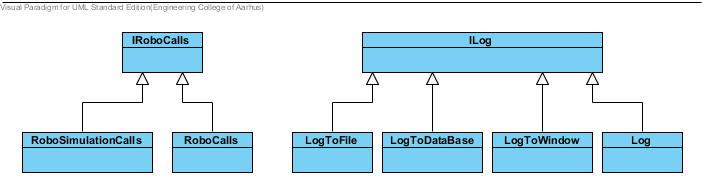
\includegraphics[scale=0.6]{Diagrammer/dSSD/Simulering/Simulering-nedarvning.jpg}
\caption{Nedarvning fra ILOG og IRoboCalls}
\end{figure}

\begin{figure}[H]
\centering
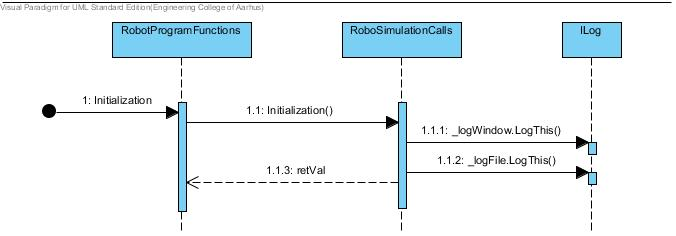
\includegraphics[scale=0.6]{Diagrammer/dSSD/Simulering/Simulering-sekvens.jpg}
\caption{Simulering Detaljeret-sekvensdiagram}
\end{figure}

\end{document}